%%%%%%%%%%%%%%%%%%%%%%%%%%%%%%%%%%%%%%%%%%%%%%%%%%%%%%%%%%%%%%%%%%
%%%                      Homework 12                           %%%
%%%%%%%%%%%%%%%%%%%%%%%%%%%%%%%%%%%%%%%%%%%%%%%%%%%%%%%%%%%%%%%%%%

\documentclass[letter]{article}

\usepackage{lipsum}
\usepackage[pdftex]{graphicx}
\usepackage[margin=1.5in]{geometry}
\usepackage[english]{babel}
\usepackage{listings}
\usepackage{amsthm}
\usepackage{amssymb}
\usepackage{framed} 
\usepackage{amsmath}
\usepackage{titling}
\usepackage{fancyhdr}

\pagestyle{fancy}


\newtheorem{theorem}{Theorem}
\newtheorem{definition}{Definition}

\newenvironment{menumerate}{%
  \edef\backupindent{\the\parindent}%
  \enumerate%
  \setlength{\parindent}{\backupindent}%
}{\endenumerate}




%%%%%%%%%%%%%%%
%% DOC INFO %%%
%%%%%%%%%%%%%%%
\newcommand{\bHWN}{12}
\newcommand{\bCLASS}{MATH H104}

\title{\bCLASS: Homework \bHWN}
\author{William Guss\\26793499\\wguss@berkeley.edu}

\fancyhead[L]{\bCLASS}
\fancyhead[CO]{Homework \bHWN}
\fancyhead[CE]{GUSS}
\fancyhead[R]{\thepage}
\fancyfoot[LR]{}
\fancyfoot[C]{}
\usepackage{csquotes}

%%%%%%%%%%%%%%

\begin{document}
\maketitle
\thispagestyle{empty}

\setcounter{section}{3}
\section{Function Spaces}

%%%%%%% Be sure to set the counter and use menumerate
\begin{menumerate}
\setcounter{enumi}{24}
	\item Prove the following.
	\begin{theorem}
		If $f: M \to M$ be a contraction and $M$ a metric space, then $f$ is uniformly continuous. 
	\end{theorem}
	\begin{proof}
		If $f$ is a contraction, then we have that there exists a $k < 1$ such that for every $x,y \in M$ $d(fx,fy) \leq kd(x,y).$ We wish to show that for every $\epsilon > 0$
		there exists a $\delta$ such that $d(x,t) <\delta$ implies $d(fx,ft) < \epsilon.$ Taking delta to be $\epsilon/k$ we have that $d(x,t) < \epsilon/k$ implies that $$d(fx,ft) \leq kd(x,y) < k\delta = \epsilon. $$
		Therefore $f$ is uniformly continuous.
	\end{proof}
	\begin{theorem}
		The extension of $f$ to the completion of $M$, denoted $M^*$, say $g: M^*\to M^*$ is a unique contraction.
	\end{theorem}
	\begin{proof}
		Recall that the completion of a metric space $(M,d) $is specifically, a pair consisiting of the completed metric space $(M^*,d^*)$ and an isometry $\phi: M \to M^*$ such that $\phi[M]$ is dense in the completed metric point set $M^*$. The extension of $f$ on the compelted metric space $(M^*, d)$ must therefore have the following property: $\phi[f(M)]$ is dense in $f^*(M^*)$. 

		First we show that an extension of a uniformly continuous function $f$ must therefore be uniformly continuous. For every $\epsilon > 0$ there exists a $\delta > 0$ such that $x,y \in M$ and $0< d(x,y) < \delta$ implies that $d(fx,fy) = d(f^*x,f^*y) < \epsilon.$ Take $x^*, y^* \in M$ with $d(x^*, y^*) < \delta(\epsilon).$ Let $$\theta(\epsilon) = \frac{\delta - d(x,y)}{4}.$$ Observe that $d(x,y) + 2\theta(\epsilon) < \delta.$ Then take $x_n,y_n \in M$ such that $d(x_n,x^*) < \theta(\epsilon)/n$ and $d(y_n,y^*) < \theta(\epsilon)/n.$ Then for all $n \in \mathbb{N}$
		$$d(x_n, y_n) < d(x_n, x^*) + d(x^*, y^*) + d(y^*, y_n) < d(x^*, y^*) + 2\theta(\epsilon) < \delta.$$
		So we have that $d(f^*x_n, f^*y_n) < \epsilon.$ Finally observe that $x_n \to x^*$ and $y_n \to y^*$ as far as convergence is concerned in $M^*.$ Since for all $n$ we have that the functional composition of the sequence is less than $\epsilon,$ sureley we must have that the extension composed with $x^*, y^*$ is less than $\epsilon.$

		In particular such satisfying $\delta = \epsilon/k$ and so $d(f^*x^*, f^*y^*) \leq kd(x^*,y^*) < \epsilon$ is a contraction. Uniqueness follows from exercise $54(b)$ of Homework $4$.
	\end{proof}
	\item Consider the following example. Let $M = (-1,0)\cup(0,1).$ Then let $f:M\to M$ such that $x \mapsto \frac12 x.$ Then $f^n(M) = (-(\frac12)^n,0)\cup(0,(\frac12)^n).$
	Suppose that there were a fixed point in $M$, say $x.$ Since $x \neq 0$, $|x| > 0$ and there exists an $N$ such that for all $n>N$ $|x| > \frac12^n$, so $x$ does not exist past the $N$th iterate of the contraction $f$. There cannot be a fixed point.
\item We now conjecture about weak contractions.
\begin{theorem}
 Not all weak contractions are contractions.
\end{theorem}
\begin{proof}
Consider the following example. Let $M = [0,1]$ be a metric space and $f:M\to M$ such that $x \to \tanh(x-1) + 1$ be a weak contraction on $M$. 
We show that $f$ is not a contraction. Suppose for the sake of contradiction that there were a $k$ such that $|f(x) - f(y)| \leq k|x-y|$ for $k < 1$. Then
let $y = 1,$ and take $y_n \to y$ such that $y_n = \frac{n-1}{n}.$ By $f$ a contraction we have that
$$\frac{|f(x)-f(y)|}{|x-y|} = \frac{1- (\tanh(-\frac{1}{n})+1)}{1- \frac{n-1}{n}} = n\tanh\left(\frac{1}{n}\right) = -n + \frac{2n}{1 + e^{-2/n}}\leq k < 1$$
However, since $n\tanh(1/n) \to 1$ as $n\to \infty$ we have a contradiction since there must be an $N$ for which all $n>N$, $n\tanh(1/n) > k$.
\end{proof}

Furthermore, it follows that even the compactness of $M$ does not give that all weak contractions are contractions by the previous theorem. 
However, fixed point theorems hold for weak contractions as is demonstrated by the following theorem.
\begin{theorem}
	If $f: M \to M$ is a weak contraction on a compact metric space $M$, then $f$ has a unique fixed point.
\end{theorem}
\begin{proof}
	By $M$ compact and $f$ a weak contraction, we have that $f$ continuous. Therefore $f(M)$ is closed up to iteration of $f.$ 
	Observe that since $f$ is a weak contraction we have that $f^{n+1}(M) \subset f^n(M).$ So it follows that $$\bigcap_{n=1}^k f^n(M) = f^k(M).$$
	Then since the $k$th iterate of $f$ on $M$ is closed we have that the infinite intersection is closed and non empty; that is,
	 $$\bigcap_{n=1}^\infty f^n(M) = F \neq \emptyset.$$

	 We claim that if $p \in F$, $p$ is a fixed point of $f.$ Suppose for the sake of contradiction that $p \notin f(F),$
	 then $f(F) \subset F$ which contradicts the fact that $\bigcap_{n=1}^\infty f^n(M) = F.$

	 Lastly we claim that $p$ is unique. Suppose there were another fixed point $q \in F.$ Then since $q\neq f$, $d(p,q) = d(fq,fp) < d(p,q)$,
	 which is a contraction, so $p$ is unique.
\end{proof}




\item Weak contractions can be brought about by limiting the derivative of real valued functions. We propose the following theorem.
\begin{figure}
  \centering
  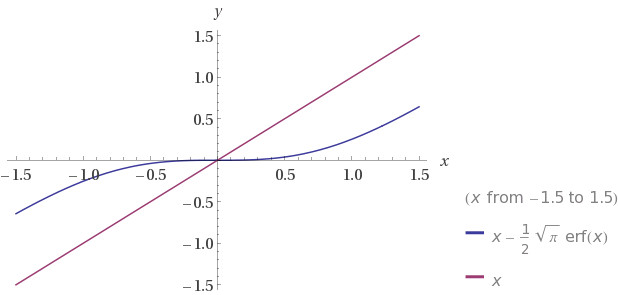
\includegraphics[width=0.75\textwidth]{28contract}
  \caption{A graph of $f:\mathbb{R}\to\mathbb{R}$ a weak contraction (but not a contraction) with $|f'(x)| < 1$ against the identity function, showing the asymtotic
  properties of the $f(x).$}
\end{figure}
\begin{theorem}
	If $f:\mathbb{R} \to \mathbb{R}$ is differentiable and is derivative satisifes $|f'(x)| < 1$ flor all $x \in \mathbb{R},$ then
	$f$ is a weak contraction.
\end{theorem}
\begin{proof}
	For any $x,y \in \mathbb{R}$ such that $x\neq y$, assume that $x < y$ without loss of generality. Then differentiability of $f$ implies that 
	for some $\theta$ between $x$ and $y,$ $$d(fx,fy) = f(\theta)d(x,y),$$ and since $f(\theta) < 1$ it is clear that $d(fx,fy) < d(x,y).$ So it follows
	that at least, $f$ is a weak contraction.
\end{proof}
Although this property of the derivative guarentees that $f$ is a weak contraciton, it does not necisarrily follow that
 $f$ is a contraction nor that it has fixed points. Consider the following example.

Let $f:\mathbb{R} \to \mathbb{R}$ such that $f'(x)$ has the property that $|f'(x)| < 1.$ In particular let $f'(x) = 1 - e^{-x^2}.$ This furthermore
gives $f$ the property that $f'(x) \to 1, x \to \infty.$ 

Clearly $f$ is a weak contraction by the theorem above, but it does not have the property of 
contraction by the following logic. Suppose that there were a $k < 1$ such that $d(fx,fy) \leq kd(x,y).$ Observe that by $f$ differentiable, we have that
for $x,y$ different $d(fx,fy) = f'(\theta)d(x,y)$ where $\theta$ is a real number between $x$ and $y.$ Since however as $x,y \to \infty$, $f'(\theta) \to 1$
we may choose $x,y$ large enough that $f'(\theta) > k,$ and we have contradicted the relationship given by contraction.

Furthermore since there are infiniteley many such $f$ satisfying the above properties, take 
$$f(x) = x - \int_0^x e^{-t^2}\ dt + 420.$$
In this case, there does not exist an $x$ such that $f(x) = x$, since $f(x) - x > 0$ for all $x.$
That is, $$\inf_{x\in \mathbb{R}}\left(420 - \int_0^x e^{-t^2}\ dt\right) = 419 > 0.$$ 
So $f$ has no fixed points even though $|f'(x)| < 1$ for all $x.$



\item We find an interesting counter example to the uniqueness of fixed points in Bruowers Fixed-Point Theorem.
\begin{theorem}
	Suppose that $f:B^m \to B^m$ is continuous where $B^m$ is the closed unit ball in $\mathbb{R}^m.$ Then although $f$ has 
	a fixed point, this point need not be unique.
\end{theorem}
\begin{proof}
	We give a simple proof by example! Take $f$ as above such that $x \mapsto x.$ Then for every $x\in B^m$, $f(x) = x$ is a fixed point.
	Therefore $f^n(x) = x$ for all $n$ and $f^n(x) \to x$ as $n \to \infty.$ So there is no unique fixed point.
\end{proof}
\end{menumerate}

\end{document}